\newpage
\section{Theoretische Grundlagen}
\label{sec:grundlagen}
%zugrundeliegende Theorien und Modelle
% Definitionen
% Stand der Technik, Normen und Standards, Wirtschaftliche Aspekte
% persönliche Positionierung

\subsection{Verdickermittel}

\subsection{Dosierstrom}

\subsubsection*{Bestimmung der Strömungsform}

Um den Dosierstrom entsprechend seiner Strömungseigenschaften charakterisieren zu können, wird zunächst mit der sogenannten \textsc{Reynoldszahl} die Strömungsform bestimmt. Sie ist eine dimensionslose Kennzahl und beschreibt das Verhältnis zwischen Tragheitskräften zu Reibungskräften in strömenden Flüssigkeiten und ist für durchströmte Rohrleitungen unter Gleichung \eqref{eq: reynolds} definiert. \cite{Foth.2014}

\begin{equation}
	\label{eq: reynolds}
	Re = \frac{d_H*\rho*\overline{u}}{\eta}
\end{equation}
\begin{parameter}
	Re 			& 	\textsc{Reynoldszahl} \\
	\eta 		& dynamische Viskosität des Fluids\\
	\rho 		& Dichte des Fluids\\
	d_H			&	hydraulischer Rohrdurchmesser\\
	\overline{u} & mittlere Strömungsgeschwindigkeit\\
\end{parameter}

Anhand der Reynoldszahl lässt sich nun mithilfe der Tabelle \ref{tab:stromung_reynolds}, die jeweilige Strömungsform zuordnen. Diese Zuordnung ist wichtig, da sich je nach Strömungsform unterschiedliche Einflussgrößen auf den Druckverlust ergeben. Beispielsweise hat für eine laminare Strömung die Wandrauigkeit der Leitung aufgrund keinen Einfluss mehr, wohin gegen sie in turbulenten Strömungen maßgebliche Druckverluste hervorrufen kann. In laminaren Strömungen überwiegt hierbei der glättende Einfluss der Viskosität gegenüber den Rohrunebenheiten, während in turbulenten Strömungen weitere Wirbel erzeugt werden. \cite{Bschorer.2018}

% Table generated by Excel2LaTeX from sheet 'Daten'
\begin{table}[h!]
	\renewcommand*{\arraystretch}{1.2}
	\centering
	\rowcolors{2}{white}{gray!25}
	\caption{Strömungsformen und ihre Reynoldszahlen \cite{Foth.2014}}
	\label{tab:stromung_reynolds}
	%\resizebox{10.5cm}{!}{
		\begin{tabulary}{1.0\textwidth}{C|CCC}
			\hline
			\textbf{Strömungsform} & \textbf{Laminar} & \textbf{Übergangsbereich} & \textbf{Turbulent}\\
			\hline
			\textbf{Reynoldszahl} &	$< 2300$ & $2300$ bis $4000$& $>4000$\\
			\hline			
	\end{tabulary}
%}
\end{table}%
\FloatBarrier

\subsubsection*{Bestimmung des Druckverlustes}
Nach der Bestimmung der Reynoldszahl lässt sich nun mit Hilfe des \linebreak \textsc{Nikuradse-Colebrook-Moody}-Diagramms, nachfolgend \textsc{Moody}-Diagramm genannt, der Rohrreibungsbeiwert $\lambda$ bestimmen (siehe Abb. \ref{fig:moody}). Dieser Wert wiederum kann in Gleichung \eqref{eq:druckverlustbeiwert} eingesetzt werden um den Druckverlustbeiwert $\zeta_R$ für gerade Rohrleitungen zu bestimmen und lässt auf Basis der erweiterten \textsc{Bernoulli}-Gleichung \eqref{eq:druckverlust_zeta} den kinetischen Druckverlust $\Delta p$ berechnen. \cite{Bschorer.2018}

\begin{equation}
	\label{eq:druckverlustbeiwert}
	\zeta_R = \lambda * \frac{L}{d}
\end{equation}
\begin{equation}
	\label{eq:druckverlust_zeta}
	\Delta p = \frac{1}{2}*\zeta_R*\rho*\overline{u}^2
\end{equation}
\begin{parameter}
	\zeta_R		& Druckverlustbeiwert für gerade Rohrstrecken\\
	L 			& Rohrleitungslänge\\
	d			& Rohrdurchmesser\\
	\Delta p	& Druckverlust \\
	\rho 			& Dichte des Fluids\\
	\overline{u} 	& mittlere Strömungsgeschwindigkeit\\
\end{parameter}


\begin{figure}[h!]
	\centering
	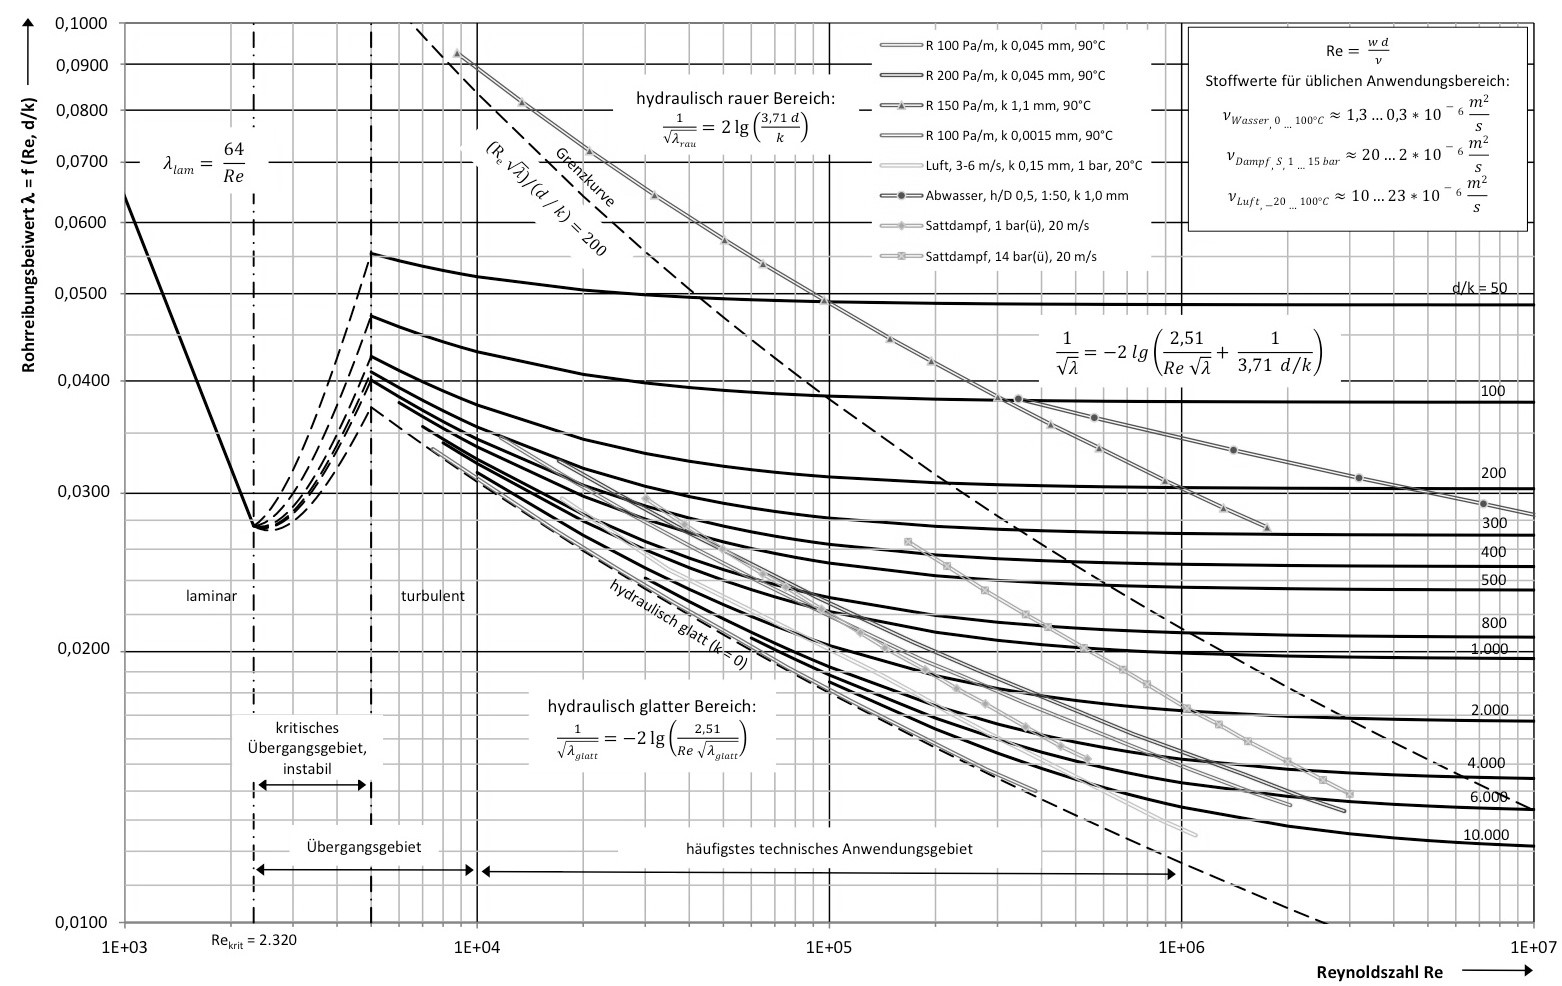
\includegraphics[width=1.0\textwidth]{img/R_Rohrreibungsbeiwert.jpg}
	\caption{\textsc{Nikuradse-Colebrook-Moody}-Diagramm \cite{Msimca.2017}}
	\label{fig:moody}
\end{figure}
\FloatBarrier
%Ende

\subsubsection*{Gesetz von  \textsc{Hagen}-\textsc{Poiseuille}}
Liegt für eine nicht-kompressible Flüssigkeit eine laminare Strömung vor, so ist es möglich die zuvor beschriebene Vorgehensweise zu vereinfachen und den auftretenden Druckverlust in der Rohrleitung direkt mit dem Gesetz von \textsc{Hagen}-\textsc{Poiseuille} zu bestimmen.  Der Druckverlust wird hierbei in Abhängigkeit vom Volumenstrom, der Rohrleitungslänge, des Rohrdurchmessers und der Viskosität berechnet. Die Definition des Gesetzes, aufgelöst nach dem Druckverlust, findet sich unter Gleichung \eqref{eq:hagen}. \cite{Foth.2005}

\begin{equation}
	\label{eq:hagen}
	\Delta p  = \frac{8*\eta*L*\dot{V}}{r^4*\pi}
\end{equation}
\begin{parameter}
	\Delta p	& Druckverlust \\
	\eta 		& dynamische Viskosität des Fluids\\
	\dot{V}		& Volumenstrom des Fluids\\
	r			& innerer Radius der Rohrleitung\\
	L 			& Rohrleitungslänge\\
\end{parameter}

Da das Gesetz von \textsc{Hagen}-\textsc{Poiseuille} bereits im \textsc{Moody}-Diagramm enthalten ist, können beide Vorgehensweisen genutzt werden um die jeweils andere Rechnung zu überprüfen. Sollen Rohrleitungseinbauten wie Armaturen, Ventile oder Bogenstücke einberechnet werden, vereinfacht jedoch aufgrund von tabellierten Druckverlustbeiwerten möglicher Einbauten die erweiterte \textsc{Bernoulli}-Gleichung die Berechnung des Druckverlustes.



\subsection{Stand der Technik}
\subsection{Dosierpumpen}
\subsubsection{oszillierende Verdrängerpumpen}
\subsubsection{rotierende Verdrängerpumpen}

\subsection{Normen und Standards}

\subsection{Rotationsviskosimeter}
\subsection{Densimeter}

Norm für Viskositätsbestimmung

https://www.din.de/de/neuer-inhalt/wdc-beuth:din21:306904236
https://www.din.de/de/wdc-beuth:din21:512291
https://www.din.de/de/neuer-inhalt/wdc-beuth:din21:329765890

\subsection{Wirtschaftliche Aspekte und Entwicklungsperspektiven}